% Options for packages loaded elsewhere
\PassOptionsToPackage{unicode}{hyperref}
\PassOptionsToPackage{hyphens}{url}
\PassOptionsToPackage{dvipsnames,svgnames,x11names}{xcolor}
%
\documentclass[
  a4paper,
  DIV=11,
  numbers=noendperiod]{scrartcl}

\usepackage{amsmath,amssymb}
\usepackage{iftex}
\ifPDFTeX
  \usepackage[T1]{fontenc}
  \usepackage[utf8]{inputenc}
  \usepackage{textcomp} % provide euro and other symbols
\else % if luatex or xetex
  \usepackage{unicode-math}
  \defaultfontfeatures{Scale=MatchLowercase}
  \defaultfontfeatures[\rmfamily]{Ligatures=TeX,Scale=1}
\fi
\usepackage{lmodern}
\ifPDFTeX\else  
    % xetex/luatex font selection
    \setmainfont[]{Noto Serif}
\fi
% Use upquote if available, for straight quotes in verbatim environments
\IfFileExists{upquote.sty}{\usepackage{upquote}}{}
\IfFileExists{microtype.sty}{% use microtype if available
  \usepackage[]{microtype}
  \UseMicrotypeSet[protrusion]{basicmath} % disable protrusion for tt fonts
}{}
\makeatletter
\@ifundefined{KOMAClassName}{% if non-KOMA class
  \IfFileExists{parskip.sty}{%
    \usepackage{parskip}
  }{% else
    \setlength{\parindent}{0pt}
    \setlength{\parskip}{6pt plus 2pt minus 1pt}}
}{% if KOMA class
  \KOMAoptions{parskip=half}}
\makeatother
\usepackage{xcolor}
\setlength{\emergencystretch}{3em} % prevent overfull lines
\setcounter{secnumdepth}{5}
% Make \paragraph and \subparagraph free-standing
\makeatletter
\ifx\paragraph\undefined\else
  \let\oldparagraph\paragraph
  \renewcommand{\paragraph}{
    \@ifstar
      \xxxParagraphStar
      \xxxParagraphNoStar
  }
  \newcommand{\xxxParagraphStar}[1]{\oldparagraph*{#1}\mbox{}}
  \newcommand{\xxxParagraphNoStar}[1]{\oldparagraph{#1}\mbox{}}
\fi
\ifx\subparagraph\undefined\else
  \let\oldsubparagraph\subparagraph
  \renewcommand{\subparagraph}{
    \@ifstar
      \xxxSubParagraphStar
      \xxxSubParagraphNoStar
  }
  \newcommand{\xxxSubParagraphStar}[1]{\oldsubparagraph*{#1}\mbox{}}
  \newcommand{\xxxSubParagraphNoStar}[1]{\oldsubparagraph{#1}\mbox{}}
\fi
\makeatother

\usepackage{color}
\usepackage{fancyvrb}
\newcommand{\VerbBar}{|}
\newcommand{\VERB}{\Verb[commandchars=\\\{\}]}
\DefineVerbatimEnvironment{Highlighting}{Verbatim}{commandchars=\\\{\}}
% Add ',fontsize=\small' for more characters per line
\usepackage{framed}
\definecolor{shadecolor}{RGB}{241,243,245}
\newenvironment{Shaded}{\begin{snugshade}}{\end{snugshade}}
\newcommand{\AlertTok}[1]{\textcolor[rgb]{0.68,0.00,0.00}{#1}}
\newcommand{\AnnotationTok}[1]{\textcolor[rgb]{0.37,0.37,0.37}{#1}}
\newcommand{\AttributeTok}[1]{\textcolor[rgb]{0.40,0.45,0.13}{#1}}
\newcommand{\BaseNTok}[1]{\textcolor[rgb]{0.68,0.00,0.00}{#1}}
\newcommand{\BuiltInTok}[1]{\textcolor[rgb]{0.00,0.23,0.31}{#1}}
\newcommand{\CharTok}[1]{\textcolor[rgb]{0.13,0.47,0.30}{#1}}
\newcommand{\CommentTok}[1]{\textcolor[rgb]{0.37,0.37,0.37}{#1}}
\newcommand{\CommentVarTok}[1]{\textcolor[rgb]{0.37,0.37,0.37}{\textit{#1}}}
\newcommand{\ConstantTok}[1]{\textcolor[rgb]{0.56,0.35,0.01}{#1}}
\newcommand{\ControlFlowTok}[1]{\textcolor[rgb]{0.00,0.23,0.31}{\textbf{#1}}}
\newcommand{\DataTypeTok}[1]{\textcolor[rgb]{0.68,0.00,0.00}{#1}}
\newcommand{\DecValTok}[1]{\textcolor[rgb]{0.68,0.00,0.00}{#1}}
\newcommand{\DocumentationTok}[1]{\textcolor[rgb]{0.37,0.37,0.37}{\textit{#1}}}
\newcommand{\ErrorTok}[1]{\textcolor[rgb]{0.68,0.00,0.00}{#1}}
\newcommand{\ExtensionTok}[1]{\textcolor[rgb]{0.00,0.23,0.31}{#1}}
\newcommand{\FloatTok}[1]{\textcolor[rgb]{0.68,0.00,0.00}{#1}}
\newcommand{\FunctionTok}[1]{\textcolor[rgb]{0.28,0.35,0.67}{#1}}
\newcommand{\ImportTok}[1]{\textcolor[rgb]{0.00,0.46,0.62}{#1}}
\newcommand{\InformationTok}[1]{\textcolor[rgb]{0.37,0.37,0.37}{#1}}
\newcommand{\KeywordTok}[1]{\textcolor[rgb]{0.00,0.23,0.31}{\textbf{#1}}}
\newcommand{\NormalTok}[1]{\textcolor[rgb]{0.00,0.23,0.31}{#1}}
\newcommand{\OperatorTok}[1]{\textcolor[rgb]{0.37,0.37,0.37}{#1}}
\newcommand{\OtherTok}[1]{\textcolor[rgb]{0.00,0.23,0.31}{#1}}
\newcommand{\PreprocessorTok}[1]{\textcolor[rgb]{0.68,0.00,0.00}{#1}}
\newcommand{\RegionMarkerTok}[1]{\textcolor[rgb]{0.00,0.23,0.31}{#1}}
\newcommand{\SpecialCharTok}[1]{\textcolor[rgb]{0.37,0.37,0.37}{#1}}
\newcommand{\SpecialStringTok}[1]{\textcolor[rgb]{0.13,0.47,0.30}{#1}}
\newcommand{\StringTok}[1]{\textcolor[rgb]{0.13,0.47,0.30}{#1}}
\newcommand{\VariableTok}[1]{\textcolor[rgb]{0.07,0.07,0.07}{#1}}
\newcommand{\VerbatimStringTok}[1]{\textcolor[rgb]{0.13,0.47,0.30}{#1}}
\newcommand{\WarningTok}[1]{\textcolor[rgb]{0.37,0.37,0.37}{\textit{#1}}}

\providecommand{\tightlist}{%
  \setlength{\itemsep}{0pt}\setlength{\parskip}{0pt}}\usepackage{longtable,booktabs,array}
\usepackage{calc} % for calculating minipage widths
% Correct order of tables after \paragraph or \subparagraph
\usepackage{etoolbox}
\makeatletter
\patchcmd\longtable{\par}{\if@noskipsec\mbox{}\fi\par}{}{}
\makeatother
% Allow footnotes in longtable head/foot
\IfFileExists{footnotehyper.sty}{\usepackage{footnotehyper}}{\usepackage{footnote}}
\makesavenoteenv{longtable}
\usepackage{graphicx}
\makeatletter
\newsavebox\pandoc@box
\newcommand*\pandocbounded[1]{% scales image to fit in text height/width
  \sbox\pandoc@box{#1}%
  \Gscale@div\@tempa{\textheight}{\dimexpr\ht\pandoc@box+\dp\pandoc@box\relax}%
  \Gscale@div\@tempb{\linewidth}{\wd\pandoc@box}%
  \ifdim\@tempb\p@<\@tempa\p@\let\@tempa\@tempb\fi% select the smaller of both
  \ifdim\@tempa\p@<\p@\scalebox{\@tempa}{\usebox\pandoc@box}%
  \else\usebox{\pandoc@box}%
  \fi%
}
% Set default figure placement to htbp
\def\fps@figure{htbp}
\makeatother

\KOMAoption{captions}{tableheading}
\usepackage{fvextra}
\DefineVerbatimEnvironment{Highlighting}{Verbatim}{breaklines,commandchars=\\\{\}}
\makeatletter
\@ifpackageloaded{caption}{}{\usepackage{caption}}
\AtBeginDocument{%
\ifdefined\contentsname
  \renewcommand*\contentsname{Table of contents}
\else
  \newcommand\contentsname{Table of contents}
\fi
\ifdefined\listfigurename
  \renewcommand*\listfigurename{List of Figures}
\else
  \newcommand\listfigurename{List of Figures}
\fi
\ifdefined\listtablename
  \renewcommand*\listtablename{List of Tables}
\else
  \newcommand\listtablename{List of Tables}
\fi
\ifdefined\figurename
  \renewcommand*\figurename{Figure}
\else
  \newcommand\figurename{Figure}
\fi
\ifdefined\tablename
  \renewcommand*\tablename{Table}
\else
  \newcommand\tablename{Table}
\fi
}
\@ifpackageloaded{float}{}{\usepackage{float}}
\floatstyle{ruled}
\@ifundefined{c@chapter}{\newfloat{codelisting}{h}{lop}}{\newfloat{codelisting}{h}{lop}[chapter]}
\floatname{codelisting}{Listing}
\newcommand*\listoflistings{\listof{codelisting}{List of Listings}}
\makeatother
\makeatletter
\makeatother
\makeatletter
\@ifpackageloaded{caption}{}{\usepackage{caption}}
\@ifpackageloaded{subcaption}{}{\usepackage{subcaption}}
\makeatother

\usepackage{bookmark}

\IfFileExists{xurl.sty}{\usepackage{xurl}}{} % add URL line breaks if available
\urlstyle{same} % disable monospaced font for URLs
\hypersetup{
  pdftitle={Laboratory 03},
  colorlinks=true,
  linkcolor={blue},
  filecolor={Maroon},
  citecolor={Blue},
  urlcolor={Blue},
  pdfcreator={LaTeX via pandoc}}


\title{Laboratory 03}
\author{}
\date{}

\begin{document}
\maketitle

\renewcommand*\contentsname{Table of contents}
{
\hypersetup{linkcolor=}
\setcounter{tocdepth}{3}
\tableofcontents
}

\section{Reply on the feedback of Lab
2}\label{reply-on-the-feedback-of-lab-2}

Thanks for the feedback on my Lab 2 Assignment! Here's my response:

\subsection{\texorpdfstring{\emph{Normally} on Line 4, Section 3.2
Question 2, Page
5}{Normally on Line 4, Section 3.2 Question 2, Page 5}}\label{normally-on-line-4-section-3.2-question-2-page-5}

\begin{quote}
``normally'' have higher median?
\end{quote}

What I mean is that based on the sample and the box-plot, we can
generally infer that ``cat people tend to have a higher life
satisfaction score'' than fish owners.

Apologies for the earlier miswording and ambiguity in the
interpretation.

\subsection{About the cats}\label{about-the-cats}

They usually come out in the early morning and late at night, as cats
\emph{normally} do. However, they are all around at various times. I
even once witnessed the police and firefighters at our faculty, rescuing
a young cat trapped on the roof!

\section{Main scenario story
(Context)}\label{main-scenario-story-context}

\begin{figure}[H]

{\centering \pandocbounded{
\includegraphics[keepaspectratio]{./health-safety.jpg}}

}

\caption{Warning - Health and Safety}

\end{figure}%

There are reports of increases in injuries related to playing games
consoles. These injuries were attributed mainly to muscle and tendon
strains. A researcher collected data from 120 participants who played on
a Nintendo Switch or watched others playing. The outcome was a pain
score from 0 to 10, where 0 is no pain and 10 is severe pain. The data
are in \texttt{switch.sav}.

\section{Main scenario quests
(Objectives)}\label{main-scenario-quests-objectives}

\begin{enumerate}
\def\labelenumi{\arabic{enumi}.}
\tightlist
\item
  Describe the distribution of the pain scores. Do you think the
  one-sample \(𝑡\) test is suitable for this variable?
\item
  A pain score of 2 is considered as minor pain. Test whether the mean
  pain score is equal to 2 (two tailed, 5\% level) and obtain the
  corresponding effect size.
\item
  Obtain a 95\% confidence interval for the mean pain score.
\item
  Summary your findings from the previous questions in several
  sentences.
\item
  (Extra credit) Obtain a 95\% confidence interval for the mean pain
  score of those who played on a Nintendo Switch. That is, exclude those
  who only watched others playing. (Hint: You learned how to exclude
  cases in Laboratory Assignment 1.)
\end{enumerate}

\section{Solutions}\label{solutions}

\subsection{A peek on the dataset}\label{a-peek-on-the-dataset}

As usual, I load modules that I may need in this laboratory assignment,
then the dataset to my RAM and check attributes of the given dataset.

\begin{Shaded}
\begin{Highlighting}[numbers=left,,]
\ImportTok{import}\NormalTok{ pandas }\ImportTok{as}\NormalTok{ pd}

\CommentTok{\# Load the dataset}
\NormalTok{switch }\OperatorTok{=}\NormalTok{ pd.read\_spss(}\StringTok{\textquotesingle{}./datasets/switch.sav\textquotesingle{}}\NormalTok{)}
\end{Highlighting}
\end{Shaded}

\begin{Shaded}
\begin{Highlighting}[numbers=left,,]
\CommentTok{\# Descriptions}
\BuiltInTok{print}\NormalTok{(}\SpecialStringTok{f\textquotesingle{}Shape: }\CharTok{\textbackslash{}n}\SpecialStringTok{\textquotesingle{}}\NormalTok{, switch.shape, }\StringTok{\textquotesingle{}}\CharTok{\textbackslash{}n}\StringTok{\textquotesingle{}}\NormalTok{)}
\BuiltInTok{print}\NormalTok{(}\SpecialStringTok{f\textquotesingle{}Columns: }\CharTok{\textbackslash{}n}\SpecialStringTok{\textquotesingle{}}\NormalTok{, switch.columns, }\StringTok{\textquotesingle{}}\CharTok{\textbackslash{}n}\StringTok{\textquotesingle{}}\NormalTok{)}
\BuiltInTok{print}\NormalTok{(}\SpecialStringTok{f\textquotesingle{}First 5 rows: }\CharTok{\textbackslash{}n}\SpecialStringTok{\textquotesingle{}}\NormalTok{, switch.head(}\DecValTok{5}\NormalTok{), }\StringTok{\textquotesingle{}}\CharTok{\textbackslash{}n}\StringTok{\textquotesingle{}}\NormalTok{)}
\BuiltInTok{print}\NormalTok{(}\SpecialStringTok{f\textquotesingle{}Describe the column \textasciigrave{}injury\textasciigrave{}: }\CharTok{\textbackslash{}n}\SpecialStringTok{\textquotesingle{}}\NormalTok{, switch.describe(), }\StringTok{\textquotesingle{}}\CharTok{\textbackslash{}n}\StringTok{\textquotesingle{}}\NormalTok{)}
\end{Highlighting}
\end{Shaded}

\begin{verbatim}
Shape: 
 (120, 5) 

Columns: 
 Index(['id', 'athlete', 'stretch', 'switch', 'injury'], dtype='object') 

First 5 rows: 
     id  athlete     stretch          switch  injury
0  ytv  Athlete  Stretching  Playing switch     2.0
1  wel  Athlete  Stretching  Playing switch     2.0
2  qfs  Athlete  Stretching  Playing switch     1.0
3  oln  Athlete  Stretching  Playing switch     2.0
4  wxi  Athlete  Stretching  Playing switch     0.0 

Describe the column `injury`: 
            injury
count  120.000000
mean     2.891667
std      1.994934
min      0.000000
25%      2.000000
50%      2.000000
75%      4.000000
max     10.000000 
\end{verbatim}

\subsection{Q1: Distribution of the pain
scores}\label{q1-distribution-of-the-pain-scores}

\subsubsection{Q1a: Describe the
distribution}\label{q1a-describe-the-distribution}

\textbf{Answer}

To describe the distribution of the pain scores, I use histogram with a
kernel density estimation curve as shown in
Figure~\ref{fig-injury-histogram} as well as measurements (mean, mode
and median) reflect central tendency (see Table~\ref{tbl-centrality}).

\begin{longtable}[]{@{}ll@{}}
\caption{Mean, mode and median}\label{tbl-centrality}\tabularnewline
\toprule\noalign{}
Measurement & Value \\
\midrule\noalign{}
\endfirsthead
\toprule\noalign{}
Measurement & Value \\
\midrule\noalign{}
\endhead
\bottomrule\noalign{}
\endlastfoot
Mode & 2.00 \\
Mean & 2.89 \\
Median & 2.00 \\
\end{longtable}

According to the graph:

\begin{enumerate}
\def\labelenumi{\arabic{enumi}.}
\tightlist
\item
  Most of the observations are clustered around the lower pain scores
  (between 1 and 4), we can say that the distribution of pain scores is
  positively skewed rather than a perfect normal distribution.
\item
  There is a noticeable peak at a score of 2, which means the most
  frequent score is around 2.
\item
  A long tail extends to the higher scores, indicating the frequency of
  pain scores gradually decreases as the scores increase.
\end{enumerate}

\textbf{Solution}

\begin{Shaded}
\begin{Highlighting}[numbers=left,,]
\NormalTok{injury }\OperatorTok{=}\NormalTok{ switch[}\StringTok{\textquotesingle{}injury\textquotesingle{}}\NormalTok{]}

\CommentTok{\# Calculate measurements of central tendency}
\NormalTok{injury\_mean }\OperatorTok{=}\NormalTok{ injury.mean()}
\NormalTok{injury\_mode }\OperatorTok{=}\NormalTok{ injury.mode()[}\DecValTok{0}\NormalTok{]}
\NormalTok{injury\_median }\OperatorTok{=}\NormalTok{ injury.median()}

\CommentTok{\# Tell the result}
\BuiltInTok{print}\NormalTok{(}\SpecialStringTok{f\textquotesingle{}Central Tendency: }\CharTok{\textbackslash{}n}\SpecialStringTok{\textquotesingle{}}\NormalTok{)}
\BuiltInTok{print}\NormalTok{(}\SpecialStringTok{f\textquotesingle{}Mean: \textquotesingle{}}\NormalTok{, injury\_mean)}
\BuiltInTok{print}\NormalTok{(}\SpecialStringTok{f\textquotesingle{}Mode: \textquotesingle{}}\NormalTok{, injury\_mode)}
\BuiltInTok{print}\NormalTok{(}\SpecialStringTok{f\textquotesingle{}Median: \textquotesingle{}}\NormalTok{, injury\_median)}
\end{Highlighting}
\end{Shaded}

\begin{verbatim}
Central Tendency: 

Mean:  2.8916666666666666
Mode:  2.0
Median:  2.0
\end{verbatim}

\begin{Shaded}
\begin{Highlighting}[numbers=left,,]
\ImportTok{import}\NormalTok{ matplotlib.pyplot }\ImportTok{as}\NormalTok{ plt}
\ImportTok{import}\NormalTok{ seaborn }\ImportTok{as}\NormalTok{ sns}

\CommentTok{\# Plot the histogram}
\NormalTok{injury\_hist }\OperatorTok{=}\NormalTok{ sns.histplot(switch, x}\OperatorTok{=}\StringTok{\textquotesingle{}injury\textquotesingle{}}\NormalTok{, stat}\OperatorTok{=}\StringTok{\textquotesingle{}count\textquotesingle{}}\NormalTok{, bins}\OperatorTok{=}\DecValTok{10}\NormalTok{ ,kde}\OperatorTok{=}\VariableTok{True}\NormalTok{)}
\CommentTok{\# Dashed line for Mean, Median and Mode}
\NormalTok{injury\_hist.axvline(injury\_mean, color}\OperatorTok{=}\StringTok{\textquotesingle{}blue\textquotesingle{}}\NormalTok{, linestyle}\OperatorTok{=}\StringTok{\textquotesingle{}{-}{-}\textquotesingle{}}\NormalTok{, linewidth}\OperatorTok{=}\DecValTok{1}\NormalTok{)}
\NormalTok{injury\_hist.axvline(injury\_median, color}\OperatorTok{=}\StringTok{\textquotesingle{}red\textquotesingle{}}\NormalTok{, linestyle}\OperatorTok{=}\StringTok{\textquotesingle{}{-}{-}\textquotesingle{}}\NormalTok{, linewidth}\OperatorTok{=}\DecValTok{1}\NormalTok{)}
\CommentTok{\# Set title and labels}
\NormalTok{injury\_hist.set\_title(}\StringTok{\textquotesingle{}Distribution of the pain scores\textquotesingle{}}\NormalTok{)}
\NormalTok{injury\_hist.set\_xlabel(}\StringTok{\textquotesingle{}Pain score (out of 10)\textquotesingle{}}\NormalTok{)}
\CommentTok{\# Show the plot}
\NormalTok{plt.show()}
\end{Highlighting}
\end{Shaded}

\begin{figure}[H]

\centering{

\pandocbounded{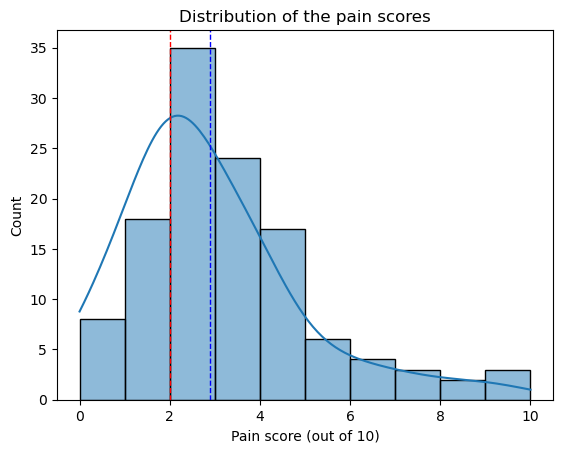
\includegraphics[keepaspectratio]{assignment_files/figure-pdf/fig-injury-histogram-output-1.png}}

}

\caption{\label{fig-injury-histogram}Distribution of the pain scores}

\end{figure}%

\subsubsection{\texorpdfstring{Q1b: One-sample \(𝑡\) test on this
variable}{Q1b: One-sample 𝑡 test on this variable}}\label{q1b-one-sample-ux1d461-test-on-this-variable}

\textbf{Answer}

Recall back the the slides in the lecture notes:

\begin{quote}
One‐sample \(t\) test requires that:

\begin{itemize}
\tightlist
\item
  Sample mean describes central tendency.
\end{itemize}
\end{quote}

The sample mean is slightly higher than the mode and median (see
Table~\ref{tbl-centrality} and Figure~\ref{fig-injury-histogram}, red
dashed lines for the median and mode, blue for the mean) since the data
is right-skewed. However, they are fairly close to each other, so the
sample mean can still represent central tendency.

\begin{quote}
\begin{itemize}
\tightlist
\item
  Scores in the sample are randomly selected from the population
\end{itemize}
\end{quote}

According to the description, the data was ``collected from 120
participants who played on a Nintendo Switch or watched others
playing.'' For the sake of this assignment, I will assume that the
participants were randomly selected from patients worldwide to fulfill
the random sampling assumption.

\begin{quote}
\begin{itemize}
\tightlist
\item
  Either \(N\) is large or \(X\) follows a normal distribution
\end{itemize}
\end{quote}

Given the right-skewed distribution as seen in
Figure~\ref{fig-injury-histogram}, the data may violate the assumption
of normality required for the one-sample \(t\)-test. However, the
\emph{Central Limit Theorem} suggests that if the sample size is large
(typically \(N > 30\)), the sampling distribution of the sample mean
tends to approach normality. Therefore, despite the skewed distribution,
the sample size (\(N = 120\)) makes the one-sample \(t\)-test acceptable
in this case.

Additionally, question 2 specifically asks for a one-sample \(t\)-test
without requiring further preprocessing of data (e.g., a log
transformation), which further supports the applicability of the
one-sample \(t\)-test to this data. If the data were unusable, there
would be no reason to include the following questions.

In conclusion, a one-sample \(t\)-test is suitable for this dataset.

\subsection{Q2: Mean of pain score
tested}\label{q2-mean-of-pain-score-tested}

\textbf{Answer}

\begin{enumerate}
\def\labelenumi{\arabic{enumi}.}
\item
  \(p\) value

  \(p \approx 3.11 \times 10^{-6}\)

  At a 5\% significance level (\(\alpha = 0.05\)), \(p < 0.001\), we
  reject the null hypothesis. The mean pain score is significantly
  different from 2 (a minor pain) at the 5\% level.
\item
  The Cohen's \(d\) value

  \(d \approx 0.45\)

  The Cohen's \(d\) value indicates a medium effect. This suggests that
  the difference between the mean pain score (\(M = 2.89\)) and the a
  minor pain (\(\mu_{hyp} = 2\)) is meaningful in practical terms.
\end{enumerate}

\textbf{Solution}

Given \(N = 120\), \(M \approx 2.89\), \(SD \approx 1.99\),
\(\mu_{hyp} = 2\), the standard error \(SE_M\) is:

\[
SE_M = \frac{SD}{\sqrt{N}} \approx 0.18
\]

\begin{Shaded}
\begin{Highlighting}[numbers=left,,]
\ImportTok{from}\NormalTok{ math }\ImportTok{import}\NormalTok{ sqrt}

\CommentTok{\# Standard Error Mean}
\CommentTok{\# Note: I can use injury.sem() directly to get the result, }
\CommentTok{\# but I shall calculate by my own for this assignment. }

\NormalTok{injury\_sem }\OperatorTok{=}\NormalTok{ injury.std(ddof}\OperatorTok{=}\DecValTok{1}\NormalTok{) }\OperatorTok{/}\NormalTok{ sqrt(}\DecValTok{120}\NormalTok{)}
\BuiltInTok{print}\NormalTok{(}\SpecialStringTok{f\textquotesingle{}Standard Error Mean: \textquotesingle{}}\NormalTok{, injury\_sem)}
\end{Highlighting}
\end{Shaded}

\begin{verbatim}
Standard Error Mean:  0.1821117309227567
\end{verbatim}

With \(SE_M \approx 0.18\), the \(t\) ratio is:

\[
t = \frac{M - \mu_{hyp}}{SE_{M}} \approx 4.90
\]

\begin{Shaded}
\begin{Highlighting}[numbers=left,,]
\CommentTok{\# t statistic}
\NormalTok{injury\_t }\OperatorTok{=}\NormalTok{ (injury.mean() }\OperatorTok{{-}} \DecValTok{2}\NormalTok{) }\OperatorTok{/}\NormalTok{ injury.sem()}
\BuiltInTok{print}\NormalTok{(}\SpecialStringTok{f\textquotesingle{}t: \textquotesingle{}}\NormalTok{, injury\_t)}
\end{Highlighting}
\end{Shaded}

\begin{verbatim}
t:  4.8962615540943375
\end{verbatim}

Unfortunately, I can't calculate the \(p\)-value on hand, so in this
part I'll call \texttt{scipy.stats.t} for help. the degree of freedom
(\(df\)) is:

\[
df = N - 1 = 120 - 1 = 119
\]

With \(t \approx 4.90\) and \(df = 119\), then use survivor function to
reach the \(p\)-value: \[
p \approx 3.11 \times 10^{-6}
\]

\begin{Shaded}
\begin{Highlighting}[numbers=left,,]
\ImportTok{import}\NormalTok{ scipy.stats }\ImportTok{as}\NormalTok{ stats}

\CommentTok{\# 119 is the degree of freedom; Two{-}sided times two}
\NormalTok{injury\_p }\OperatorTok{=}\NormalTok{ stats.t.sf(injury\_t, }\DecValTok{119}\NormalTok{ ) }\OperatorTok{*} \DecValTok{2}

\BuiltInTok{print}\NormalTok{(}\SpecialStringTok{f\textquotesingle{}p: \textquotesingle{}}\NormalTok{, injury\_p)}
\end{Highlighting}
\end{Shaded}

\begin{verbatim}
p:  3.1051091723547962e-06
\end{verbatim}

The \(p\)-value is much smaller than 0.001 (\(p < 0.001\)), the null
hypothesis should be rejected.

I also did a sanity check with the ready-to-use function
\texttt{scipy.stats.ttest\_1samp}:

\begin{Shaded}
\begin{Highlighting}[numbers=left,,]
\CommentTok{\# A san{-}check on my calculation result: }

\NormalTok{injury\_ttest\_1samp }\OperatorTok{=}\NormalTok{ stats.ttest\_1samp(injury, }\DecValTok{2}\NormalTok{, alternative}\OperatorTok{=}\StringTok{\textquotesingle{}two{-}sided\textquotesingle{}}\NormalTok{)}

\BuiltInTok{print}\NormalTok{(}\SpecialStringTok{f\textquotesingle{}t: \textquotesingle{}}\NormalTok{, injury\_ttest\_1samp.statistic, }\StringTok{\textquotesingle{}}\CharTok{\textbackslash{}n}\StringTok{\textquotesingle{}}
      \StringTok{\textquotesingle{}df: \textquotesingle{}}\NormalTok{, injury\_ttest\_1samp.df, }\StringTok{\textquotesingle{}}\CharTok{\textbackslash{}n}\StringTok{\textquotesingle{}}
      \StringTok{\textquotesingle{}p{-}value: \textquotesingle{}}\NormalTok{, injury\_ttest\_1samp.pvalue)}
\end{Highlighting}
\end{Shaded}

\begin{verbatim}
t:  4.8962615540943375 
df:  119 
p-value:  3.1051091723547962e-06
\end{verbatim}

The Cohen's d value is:

\[
d = \frac{M - \mu_{hyp}}{SD} = \frac{t}{\sqrt{N}} \approx 0.45
\]

\begin{Shaded}
\begin{Highlighting}[numbers=left,,]
\CommentTok{\# Effect Size d}

\NormalTok{injury\_d }\OperatorTok{=}\NormalTok{ injury\_t }\OperatorTok{/}\NormalTok{ sqrt(}\DecValTok{120}\NormalTok{)}
\BuiltInTok{print}\NormalTok{(}\SpecialStringTok{f\textquotesingle{}Cohen}\CharTok{\textbackslash{}\textquotesingle{}}\SpecialStringTok{s d:\textquotesingle{}}\NormalTok{, injury\_d)}
\end{Highlighting}
\end{Shaded}

\begin{verbatim}
Cohen's d: 0.4469654834371283
\end{verbatim}

\subsection{Q3: 95\% confidence interval for the mean pain
score}\label{q3-95-confidence-interval-for-the-mean-pain-score}

\textbf{Answer}

Based on the sample of \(N = 120\) pain scores, with \(M \approx 2.89\)
and \(SD \approx 1.99\), the 95\% CI for pain scores is
\([2.53, 3.25]\).

\textbf{Solution}

Given \(c = 1.96\) for a 95\% confidence interval and
\(SE_M \approx 0.18\) as calculated in the last section, a 95\%
confidence interval of the mean pain score is:

\[
[M - c \times SE_M, M + c \times SE_M] \approx [2.53, 3.25]
\]

\begin{Shaded}
\begin{Highlighting}[numbers=left,,]
\CommentTok{\# CI for two{-}tailed t{-}statistics}
\KeywordTok{def}\NormalTok{ confidence\_interval(alpha, mean, sem, df): }
\NormalTok{    c }\OperatorTok{=}\NormalTok{ stats.t.interval(}\DecValTok{1} \OperatorTok{{-}}\NormalTok{ alpha, df)[}\DecValTok{1}\NormalTok{]}
\NormalTok{    ci\_upper }\OperatorTok{=}\NormalTok{ mean }\OperatorTok{+}\NormalTok{ (c }\OperatorTok{*}\NormalTok{ sem)}
\NormalTok{    ci\_lower }\OperatorTok{=}\NormalTok{ mean }\OperatorTok{{-}}\NormalTok{ (c }\OperatorTok{*}\NormalTok{ sem)}
    \BuiltInTok{print}\NormalTok{(}\SpecialStringTok{f\textquotesingle{}CI (Lower): \textquotesingle{}}\NormalTok{, ci\_lower)}
    \BuiltInTok{print}\NormalTok{(}\SpecialStringTok{f\textquotesingle{}CI (Upper): \textquotesingle{}}\NormalTok{, ci\_upper)}
    \ControlFlowTok{return} \BuiltInTok{str}\NormalTok{(}\SpecialStringTok{f\textquotesingle{}[}\SpecialCharTok{\{}\NormalTok{ci\_lower}\SpecialCharTok{\}}\SpecialStringTok{, }\SpecialCharTok{\{}\NormalTok{ci\_upper}\SpecialCharTok{\}}\SpecialStringTok{]\textquotesingle{}}\NormalTok{)}

\NormalTok{injury\_ci }\OperatorTok{=}\NormalTok{ confidence\_interval(}\FloatTok{0.05}\NormalTok{, injury\_mean, injury\_sem, }\DecValTok{119}\NormalTok{)}
\BuiltInTok{print}\NormalTok{(injury\_ci)}
\end{Highlighting}
\end{Shaded}

\begin{verbatim}
CI (Lower):  2.53106725077079
CI (Upper):  3.252266082562543
[2.53106725077079, 3.252266082562543]
\end{verbatim}

\begin{Shaded}
\begin{Highlighting}[numbers=left,,]
\CommentTok{\# And scipy.stats.t does the same thing. }
\NormalTok{stats.t.interval(confidence}\OperatorTok{=}\FloatTok{0.95}\NormalTok{, }
\NormalTok{                 df}\OperatorTok{=}\DecValTok{119}\NormalTok{, }
\NormalTok{                 loc}\OperatorTok{=}\NormalTok{injury\_mean, }
\NormalTok{                 scale}\OperatorTok{=}\NormalTok{injury\_sem)}
\end{Highlighting}
\end{Shaded}

\begin{verbatim}
(2.53106725077079, 3.252266082562543)
\end{verbatim}

\subsection{Q4: Summarizing the
findings}\label{q4-summarizing-the-findings}

\textbf{Answer}

A one‐sample \(t\)-test is conducted to reveal whether mean pain score
for a sample of \(N = 120\) patients differed from the minor pain with a
score of 2. For this example, \(M = 2.89\), \(SD = 1.99\) and
\(SE_M = 0.18\). The 95\% CI for \(M\) was \([2.53, 3.25]\). The result
was \(t(119) = 4.90\), \(p < 0.001\), two tailed. The effect size is
\(d = 0.45\) by Cohen's standards, which represents a medium effect. The
difference between the sample mean (\(M = 2.89\)) and the score of minor
pain (2) is statistically significant using \(\alpha = 0.05\), two
tailed.

\subsection{Q5: 95\% CI for Switch players' mean pain
score}\label{q5-95-ci-for-switch-players-mean-pain-score}

\textbf{Answer}

The 95\% confidence interval for the mean pain score of those who played
on a Nintendo Switch is \([3.14, 4.33]\).

\textbf{Solution}

\begin{enumerate}
\def\labelenumi{\arabic{enumi}.}
\tightlist
\item
  Check the structure of column \texttt{switch} then apply the
  filtering:
\end{enumerate}

\begin{Shaded}
\begin{Highlighting}[numbers=left,,]
\CommentTok{\# Check how many people get injured while playing}
\BuiltInTok{print}\NormalTok{(}\SpecialStringTok{f\textquotesingle{}Variables in the column switch: }\CharTok{\textbackslash{}n}\SpecialStringTok{\textquotesingle{}}\NormalTok{, switch[}\StringTok{\textquotesingle{}switch\textquotesingle{}}\NormalTok{].value\_counts())}
\CommentTok{\# Filter out all switch players}
\NormalTok{injury\_ns }\OperatorTok{=}\NormalTok{ switch[switch[}\StringTok{\textquotesingle{}switch\textquotesingle{}}\NormalTok{] }\OperatorTok{==} \StringTok{\textquotesingle{}Playing switch\textquotesingle{}}\NormalTok{][}\StringTok{\textquotesingle{}injury\textquotesingle{}}\NormalTok{]}
\CommentTok{\# And a sanity check}
\BuiltInTok{print}\NormalTok{(}\SpecialStringTok{f\textquotesingle{}Filtered data: }\CharTok{\textbackslash{}n}\SpecialStringTok{\textquotesingle{}}\NormalTok{, injury\_ns.describe())}
\end{Highlighting}
\end{Shaded}

\begin{verbatim}
Variables in the column switch: 
 switch
Playing switch     60
Watching switch    60
Name: count, dtype: int64
Filtered data: 
 count    60.000000
mean      3.733333
std       2.313312
min       0.000000
25%       2.000000
50%       3.500000
75%       5.000000
max      10.000000
Name: injury, dtype: float64
\end{verbatim}

\begin{enumerate}
\def\labelenumi{\arabic{enumi}.}
\setcounter{enumi}{1}
\tightlist
\item
  Calculating the CI:
\end{enumerate}

Given \(N_{player} = 60\), then the
\(df_{player} = N_{player} - 1 = 59\),\\
Based on the data we also have \(M_{player} \approx 3.73\) and
\(SE_{M_{player}} \approx 0.30\)

The 95\% confidence interval for the mean pain score of those who played
on a Nintendo Switch is:

\[
[M - c \times SE_M, M + c \times SE_M] \approx [3.14, 4.33]
\]

\begin{Shaded}
\begin{Highlighting}[numbers=left,,]
\NormalTok{injury\_ns\_mean }\OperatorTok{=}\NormalTok{ injury\_ns.mean()}
\NormalTok{injury\_ns\_sem }\OperatorTok{=}\NormalTok{ injury\_ns.sem()}
\NormalTok{injury\_ns\_dregf }\OperatorTok{=} \BuiltInTok{len}\NormalTok{(injury\_ns) }\OperatorTok{{-}} \DecValTok{1}

\BuiltInTok{print}\NormalTok{(}\SpecialStringTok{f\textquotesingle{}Sample size: }\SpecialCharTok{\{}\BuiltInTok{len}\NormalTok{(injury\_ns)}\SpecialCharTok{\}}\SpecialStringTok{, }\CharTok{\textbackslash{}n}\SpecialStringTok{\textquotesingle{}}
      \SpecialStringTok{f\textquotesingle{}Degree of Freedom: }\SpecialCharTok{\{}\NormalTok{injury\_ns\_dregf}\SpecialCharTok{\}}\SpecialStringTok{,}\CharTok{\textbackslash{}n}\SpecialStringTok{\textquotesingle{}}
      \SpecialStringTok{f\textquotesingle{}Mean: }\SpecialCharTok{\{}\NormalTok{injury\_ns\_mean}\SpecialCharTok{\}}\SpecialStringTok{,}\CharTok{\textbackslash{}n}\SpecialStringTok{\textquotesingle{}}
      \SpecialStringTok{f\textquotesingle{}Standard Error: }\SpecialCharTok{\{}\NormalTok{injury\_ns\_sem}\SpecialCharTok{\}}\SpecialStringTok{\textquotesingle{}}\NormalTok{)}

\NormalTok{injury\_ns\_ci }\OperatorTok{=}\NormalTok{ confidence\_interval(}\FloatTok{0.05}\NormalTok{, injury\_ns\_mean, injury\_ns\_sem, injury\_ns\_dregf)}
\BuiltInTok{print}\NormalTok{(}\SpecialStringTok{f\textquotesingle{}}\CharTok{\textbackslash{}n}\SpecialStringTok{The 95\% CI for Switch players: }\CharTok{\textbackslash{}n}\SpecialStringTok{\textquotesingle{}}\NormalTok{, injury\_ns\_ci)}
\end{Highlighting}
\end{Shaded}

\begin{verbatim}
Sample size: 60, 
Degree of Freedom: 59,
Mean: 3.7333333333333334,
Standard Error: 0.29864729557842784
CI (Lower):  3.1357414752023387
CI (Upper):  4.3309251914643285

The 95% CI for Switch players: 
 [3.1357414752023387, 4.3309251914643285]
\end{verbatim}




\end{document}
